%==============================================================================
%  Concept poster - "Diffusion Models as Classifiers for EEG Seizure Detection"
%  An IDEA poster (no results yet). Target audience: CS PhD students.
%  Compile:  pdflatex poster_seizure_diffusion.tex   (run twice)
%  Class:    tikzposter (ships with TeX Live / MiKTeX, no extra downloads)
%==============================================================================
\documentclass[26pt, a0paper, landscape, margin=0mm, innermargin=18mm,
               blockverticalspace=14mm, colspace=26mm, subcolspace=0mm]{tikzposter}

\usepackage[utf8]{inputenc}
\usepackage{amsmath, amssymb}
\usepackage{booktabs}
\usepackage{tikz}
\usetikzlibrary{arrows.meta, positioning}

%--- Look & feel -------------------------------------------------------------
\usetheme{Default}
\usecolorstyle{Britain}

\definecolor{accent}{RGB}{0, 102, 153}
\definecolor{accent2}{RGB}{204, 85, 0}

% Consistent 3-field template for the four variant blocks
\newcommand{\variant}[3]{%
  \textbf{\color{accent}Idea.}\ #1\\[9pt]
  \textbf{\color{accent}Decision.}\ #2\\[9pt]
  \textbf{\color{accent2}Trade-off.}\ #3}

%--- Title block -------------------------------------------------------------
\title{\parbox{\linewidth}{\centering Diffusion Models as Classifiers for EEG Seizure Detection}}
\author{Annika Stiehl}
\institute{Hochschule Ansbach (HSAN) \quad$\cdot$\quad PhD Student \quad$\cdot$\quad
           \texttt{annika.stiehl@hs-ansbach.de}}

\begin{document}
\maketitle[width=0.96\linewidth]

%==============================================================================
\begin{columns}
%==============================================================================
%  LEFT TWO-THIRDS - two sub-columns (setup | pipeline+data) over a shared image box
%==============================================================================
\column{0.66}
\begin{subcolumns}
\subcolumn{0.5}

%------------------------------------------------------------------------------
\block{1.\ Motivation \& Core Question}{
  \begin{itemize}
    \item \textbf{Problem.} Epilepsy affects $\sim$1\% of people. Seizure
          detection in EEG is still done \emph{by hand} - slow, error-prone,
          hours of multi-channel data scanned window by window.
    \item \textbf{Gap.} \emph{Discriminative} CNNs/RNNs dominate; \emph{generative}
          models serve mostly for augmentation - rarely as the classifier itself,
          especially for biomedical \emph{time series}~[3].
    \item \textbf{Why generative?} A class-conditional model of the \emph{signal}
          gives a likelihood + per-window uncertainty, not just a label - so a
          clinician can trust or defer each call.
  \end{itemize}

  \medskip
  \begin{tikzfigure}
  \colorbox{accent!12}{\parbox{0.92\linewidth}{\centering\vspace{4pt}
  \textbf{Core question}\\[4pt]
  One frozen conditional diffusion model, four variants - differing only in
  \emph{how} its outputs become a decision: from \emph{training-free} (V1, V2)
  to a \emph{learned read-out} (V3, V4).\\[2pt]
  \textbf{Which mechanism detects seizures most robustly?}
  \vspace{4pt}}}
  \end{tikzfigure}
}

%------------------------------------------------------------------------------
\block{2.\ A Diffusion Model is Secretly a Classifier}{
  A \textbf{DDPM} learns to reverse a noising process; the forward step is
  \[
    x_t = \sqrt{\bar\alpha_t}\,x_0 + \sqrt{1-\bar\alpha_t}\,\epsilon .
  \]
  \begin{itemize}
    \item Schedule $\bar\alpha_t$: $1$ (signal $x_0$) $\to$ $0$ (pure noise).
    \item Network $\epsilon_\theta(x_t,t,c)$ predicts the noise, \emph{conditioned}
          on class label $c$.
    \item \textbf{Key idea} (Li et al.~[1]): pick the class whose conditioning
          best explains the observed noise.
    \item In its purest form (V1, V2) - no extra classifier, no extra training:
          the generative model \emph{is} the classifier.
  \end{itemize}
}

%------------------------------------------------------------------------------
\subcolumn{0.5}

%------------------------------------------------------------------------------
\block{3.\ How a Window Gets Classified}{
  For an EEG window $O$: add noise, then score \emph{both} class labels on the
  \emph{same} noised input.

  \medskip
  \begin{tikzfigure}
  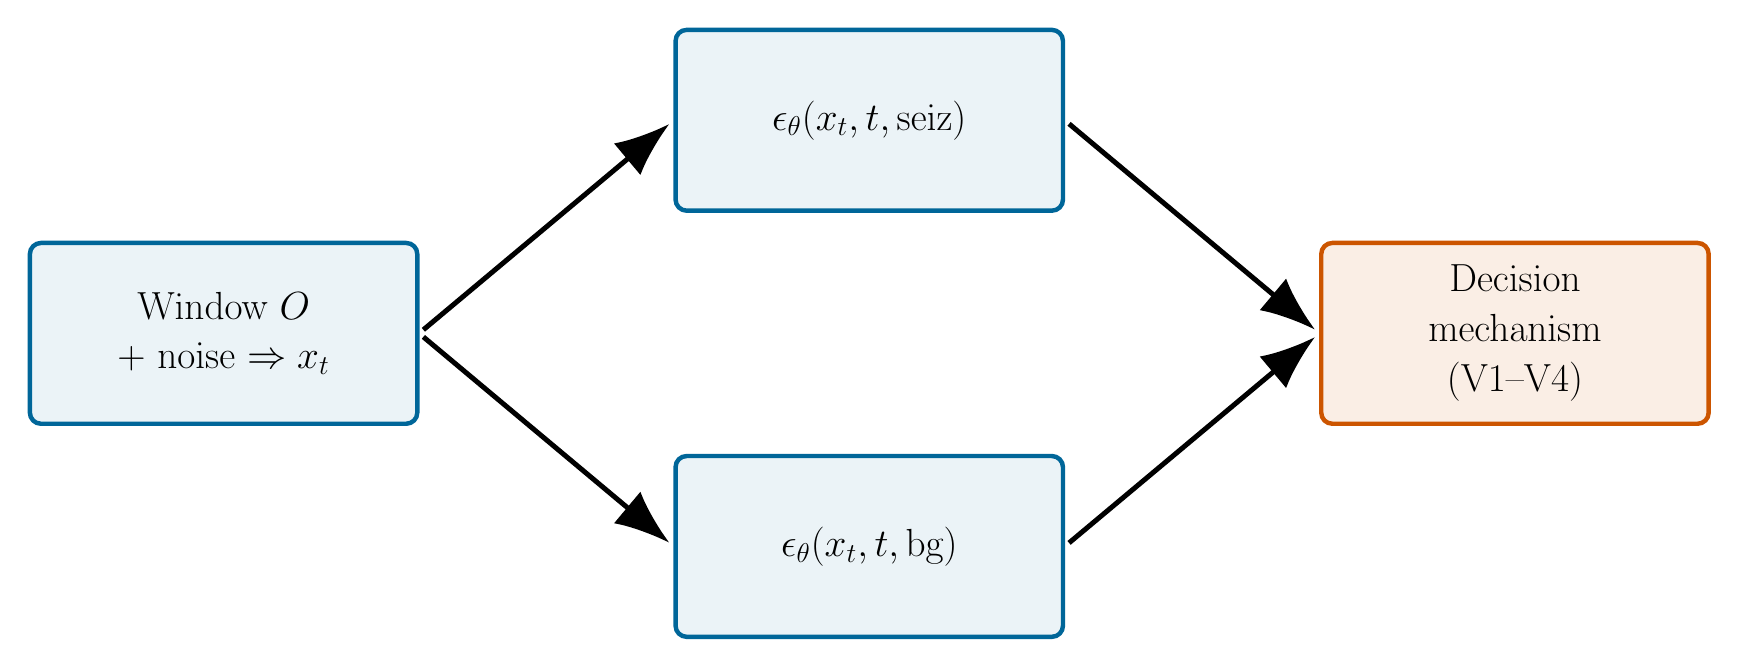
\begin{tikzpicture}[
      font=\LARGE, scale=0.82, transform shape,
      box/.style={draw=accent, line width=1.6pt, rounded corners,
                  fill=accent!8, minimum height=2.8cm, minimum width=6.0cm,
                  align=center, inner sep=9pt},
      dec/.style={draw=accent2, line width=1.6pt, rounded corners,
                  fill=accent2!10, minimum height=2.8cm, minimum width=6.0cm,
                  align=center, inner sep=9pt},
      arr/.style={-{Latex[length=7mm]}, line width=1.8pt, shorten >=2pt, shorten <=2pt}]
    \node[box] (o) at (0,0)     {Window $O$\\$+$ noise $\Rightarrow x_t$};
    \node[box] (s) at (10,3.3)  {$\epsilon_\theta(x_t,t,\text{seiz})$};
    \node[box] (b) at (10,-3.3) {$\epsilon_\theta(x_t,t,\text{bg})$};
    \node[dec] (d) at (20,0)    {Decision\\mechanism\\(V1--V4)};
    \draw[arr] (o.east) -- (s.west);
    \draw[arr] (o.east) -- (b.west);
    \draw[arr] (s.east) -- (d.west);
    \draw[arr] (b.east) -- (d.west);
  \end{tikzpicture}
  \end{tikzfigure}

  \medskip
  \begin{itemize}
    \item Repeat over random timesteps + noise (e.g.\ $N{=}50\times$) (V1), then
          aggregate per-draw scores into one decision.
  \end{itemize}
}

%------------------------------------------------------------------------------
\block{Data \& Experimental Setup}{
  \begin{itemize}
    \item \textbf{Dataset.} TUSZ v2.0.6 - largest public corpus of clinical EEG
          with expert seizure annotations.
    \item \textbf{Input.} 27-channel scalp EEG, 2\,s windows.
    \item \textbf{Task.} Binary per-window: \emph{seizure} vs.\ \emph{background}.
    \item \textbf{Protocol.} Official Temple University split - subject-disjoint
          (no patient in two splits).
    \item \textbf{Challenge.} Seizures $<$5\% per split - \emph{severe class
          imbalance}. Shapes training (few seizure examples) and evaluation
          (report sensitivity at fixed FA-rate, not only ROC-AUC / Balanced Acc.).
  \end{itemize}
}

%------------------------------------------------------------------------------
\end{subcolumns}

%------------------------------------------------------------------------------
\block{Generated EEG Signals - Conditional Samples from the Diffusion Model}{
  \centering
  Two class-conditional windows (2 seconds, 128 Hz) drawn from the trained model (epoch 85)
  $\epsilon_\theta(\cdot,\cdot,c)$ - 27 channels stacked with vertical offset. \\
  \textbf{Left:} Background; \textbf{Right:} Seizure\\[-21pt]
  \begin{tikzfigure}
    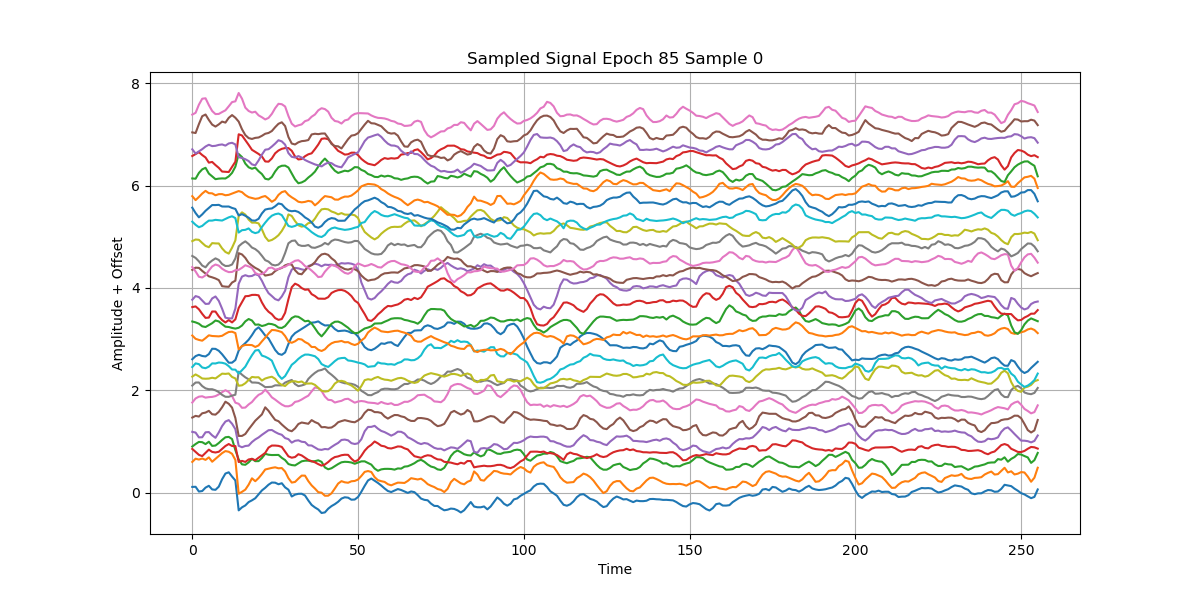
\includegraphics[trim=0 20 0 0, clip, width=0.49\linewidth]{sample_epoch5_0.png}\hspace{-3cm}
    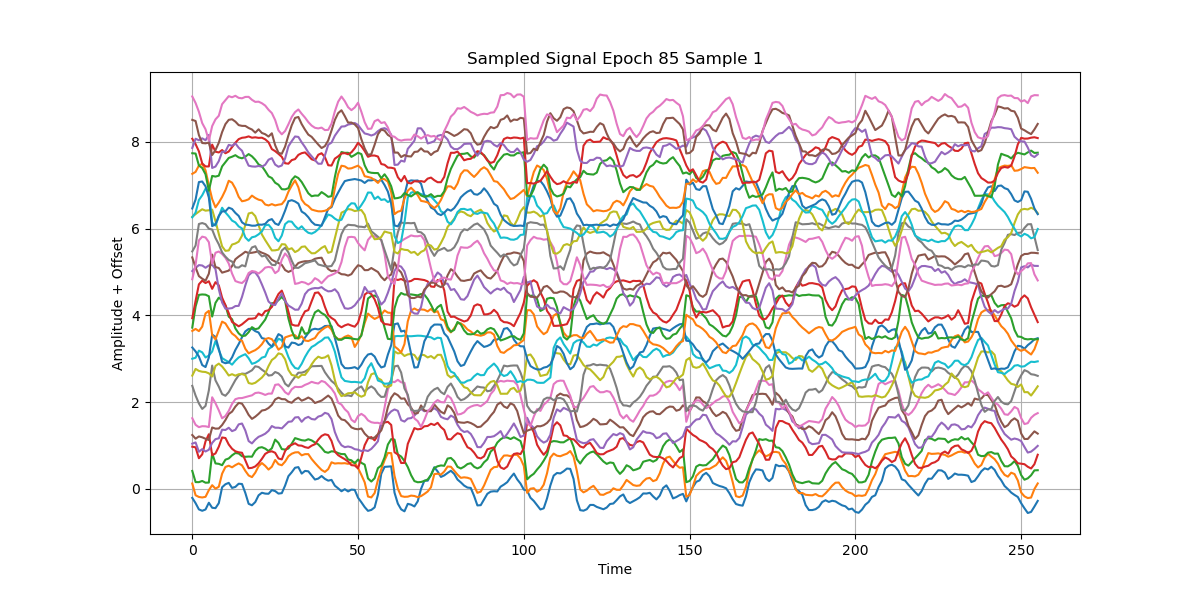
\includegraphics[trim=0 20 0 0, clip, width=0.49\linewidth]{sample_epoch5_1.png}
  \end{tikzfigure}
}

%==============================================================================
%  RIGHT THIRD - the four decision mechanisms
%==============================================================================
\column{0.34}

%------------------------------------------------------------------------------
\block{V1 - Monte-Carlo Majority Vote~[1,\,3]}{
  \variant
  {Which class label lets the denoiser better predict this window's noise?}
  {Per draw, vote for class $c$ with smaller error
   $e^{(c)}=\lVert\epsilon_\theta(x_t,t,c)-\epsilon\rVert_2^2$;
   \emph{majority} over $N$ draws.}
  {Training-free, strong baseline - but coarse, poorly-calibrated confidence;
   metric choice (MAE/MSE) open.}
}

%------------------------------------------------------------------------------
\block{V2 - Probability-Flow Log-Likelihood~[2]}{
  \variant
  {Don't count votes - measure how \emph{probable} the window is per class.}
  {Probability-flow ODE gives a \emph{numerical} log-likelihood per class; decide
   by the ratio
   $\Delta\mathrm{LL}=\log p_\theta(O|\text{seiz})-\log p_\theta(O|\text{bg})$.}
  {Optimal if densities are correct (Neyman--Pearson), best-calibrated score -
   but an ODE solve per window is costly.}
}

%------------------------------------------------------------------------------
\block{V3 - Learned Critic~[5]}{
  \variant
  {Don't hand-pick the metric - let a small model \emph{learn} what separates
   the classes.}
  {Feed diffusion outputs (predicted noise / per-step errors) to a learned critic
   (CNN or gradient-boosted) outputting $P(\text{seiz}\,|\,O)$.}
  {Most flexible $\Rightarrow$ highest accuracy potential - but needs own training
   and can overfit the model's artifacts.}
}

%------------------------------------------------------------------------------
\block{V4 - Siamese / Triplet Metric~[4]}{
  \variant
  {Learn a \emph{distance} where a window sits closer to its own class's
   generated version.}
  {Encoder trained with triplet loss $+$ hard-negative mining; classify by
   smaller \emph{average learned distance} over $N$ runs.}
  {Most expressive, gives continuous per-window uncertainty - but hardest to
   train: hard-negative mining is unstable.}
}

%------------------------------------------------------------------------------
\block{References}{
  {\small
  [1] Li et al., ICCV 2023 \,$\cdot$\,
  [2] Song et al., ICLR 2021 \,$\cdot$\,
  [3] Vetter et al., Patterns 2024 \,$\cdot$\,
  [4] Schroff et al., CVPR 2015 \,$\cdot$\,
  [5] Kim et al., ICML 2023.}
}

\end{columns}
\end{document}
